\documentclass[a4paper]{article}
\usepackage[margin=1in]{geometry}
\usepackage[english]{babel}
\usepackage[utf8]{inputenc}
\usepackage{amsmath}
\usepackage{graphicx}
\usepackage{amssymb}
\usepackage{amsthm}
\usepackage{tikz}
\usetikzlibrary{calc}
\usepackage{tikz-cd}
\usepackage{mathrsfs}
\usepackage[colorinlistoftodos]{todonotes}
\usepackage{enumitem}
\usepackage{yfonts}
\usepackage{dsfont}
\usepackage{mathtools}
\usepackage{hyperref} 
\usepackage{mathtools}
\DeclarePairedDelimiter\ceil{\lceil}{\rceil}
\DeclarePairedDelimiter\floor{\lfloor}{\rfloor}

\title{Complex Analysis Notes}
\author{Wilson Pan}
\date{\today}

\newtheorem{thm}{Theorem}[section]
\newtheorem{lem}[thm]{Lemma}
\newtheorem{defn}[thm]{Definition}
\newtheorem{eg}[thm]{Example}
\newtheorem{ex}[thm]{Exercise}
\newtheorem{conj}[thm]{Conjecture}
\newtheorem{cor}[thm]{Corollary}
\newtheorem{claim}[thm]{Claim}
\newtheorem{rmk}[thm]{Remark}

\newcommand{\ie}{\emph{i.e.} }
\newcommand{\cf}{\emph{cf.} }
\newcommand{\into}{\hookrightarrow}
\newcommand{\dirac}{\slashed{\partial}}
\newcommand{\R}{\mathbb{R}}
\newcommand{\C}{\mathbb{C}}
\newcommand{\Z}{\mathbb{Z}}
\newcommand{\N}{\mathbb{N}}
\newcommand{\Q}{\mathbb{Q}}
\newcommand{\LieT}{\mathfrak{t}}
\newcommand{\T}{\mathbb{T}}
\newcommand{\A}{\mathds{A}}
\newcommand{\HG}{\mathcal{H}}
\newcommand{\F}{\mathbb{F}}
\newcommand{\poly}[2]{\text{Poly}_{#1}(#2)}
\newcommand{\gen}[1]{\langle #1 \rangle}
\newcommand{\Hom}{\text{Hom}}
\newcommand{\E}{\mathbb{E}} 
\newcommand{\res}{\upharpoonright}
\newcommand{\diam}{\text{diam}}
\begin{document}

\maketitle

\tableofcontents
\newpage

\section{Jan 12}
\begin{defn}
    Let $\Omega$ be an open set in $\C$ and $f$ a complex-valued function on $\Omega$. A  function $f$ is holomorphic at a point $z_0\in \Omega$ if the quotient \[
    \frac{f(z_0+h)-f(z_0)}{h}
    .\] 
    converges to a limit when $h\to 0.$ The limit of the quotient, when it exists, is denoted $f'(z_0).$
\end{defn}
\begin{thm}
    A function $F(x,y)=(u(x,y),v(x,y))$ is said to be differentiable at a point $P_0(x_0,y_0)$ if there exist a linear transformation $J:\R^2\to \R^2$ such that \[
    \frac{|F(P_0+H)-F(P_0)-J(H)|}{|H|}\to 0 \text{ as } |H|\to 0
    .\] 
\end{thm}
\begin{defn}
    The jacobian matrix of $F$ is \[
    J=J_F(x,y)=\begin{pmatrix}
        {\frac{\partial u}{\partial x} } & {\frac{\partial u}{\partial y} } \\ 
        {\frac{\partial v}{\partial x} } & {\frac{\partial v}{\partial y} }
    \end{pmatrix}
    .\] 
\end{defn}
\begin{thm}
    Cauchy-Riemann Equations: If $f$ is holomorphic then 
    \[
    \frac{\partial u}{\partial x} = \frac{\partial v}{\partial y}  \text{ and } \frac{\partial u}{\partial y} =-\frac{\partial v}{\partial x} 
    .\] 
    \begin{proof}
        If we write $z=x+iy,z_0=x_0+iy_0$ and $f(z)=f(x,y)$ then 
        \begin{align*}
            f'(z_0)&=\lim_{h_1\to 0} \frac{f(x_0+h_1,y_0)-f(x_0,y_0)}{h_1}\\
            &=\frac{\partial f}{\partial x} (z_0)
        \end{align*}
        Similarly, now take $h$ purely imaginary, say $h=ih_2$, then 
        \begin{align*}
            f'(z_0)&=\lim_{h_2\to 0}  \frac{f(x_0,y_0+h_2)-f(x_0,y_0)}{ih_2}\\
            &=\frac{1}{i}\frac{\partial f}{\partial y} (z_0)
        \end{align*}
        Since $f$ is holomorphic we have \[
        \frac{\partial f}{\partial x} =\frac{1}{i}\frac{\partial f}{\partial y}
        .\] 
        Writing $f=u+iv$ we have the stated relation.
    \end{proof}
\end{thm}
\newpage
\section{Jan 14}
\begin{thm}
    $f:\Omega\to \mathbb{C}$ holomorphic on $\Omega$ equivalently $F=\begin{pmatrix}
        {u} \\ 
        {v}
    \end{pmatrix}:\R^2\to \R^2$. The partials $\frac{\partial u}{\partial x}, \frac{\partial u}{\partial y}, \frac{\partial v}{\partial x}, \frac{\partial v}{\partial y}$ exist and satisfy the Cauchy-Riemann equations \[
    \frac{\partial u}{\partial x}=\frac{\partial v}{\partial y}, \frac{\partial u}{\partial y}=-\frac{\partial v}{\partial x}
    .\] 
    Moreover, $F$ is $\R$-differentiable, there exist a linear map $\mathcal{L}:\R^2\to\R^2$ such that $F((x,y)+(h_1,h_2))-F(x,y)=\mathcal{L}(h_1,h_2)+o(h)$ \[
    \mathcal{L}=\begin{pmatrix}
        {\frac{\partial u}{\partial x}} & {\frac{\partial u}{\partial y}} \\ 
        {\frac{\partial v}{\partial x}} & {\frac{\partial v}{\partial y}}
    \end{pmatrix}
    .\]  
    \begin{proof}
        We have 
        \begin{align}
            \frac{|F((x,y)+(h_1,h_2))-F(x,y)-\mathcal{L}(h_1,h_2)|}{|h|}&=\frac{\left | \begin{pmatrix}
                {u(\overline{z}+\overline{h})-u(\overline{z})-\frac{\partial u}{\partial x}h_1-\frac{\partial u}{\partial y}h_2} \\ 
                {v(\overline{z}+\overline{h})-v(\overline{z})-\frac{\partial v}{\partial x}h_1-\frac{\partial v}{\partial y}h_2}
            \end{pmatrix}\right |}{|h|}\\
            &=\frac{|f(z+h)-f(z)-f'(z)h|}{|h|}\to 0
        \end{align}
        Where $f(z+h)=u(z+h)+iv(z+h)$, $f(z)=u(z)+iv(z)$ and $f'(z)=\frac{\partial u }{\partial x}+i \frac{\partial v }{\partial x}$.
    \end{proof}
\end{thm}
\begin{cor}
    $f$ holomorphic implies $F$ is $\R$-differentiable. Let $a=\frac{\partial u }{\partial x}=\frac{\partial v}{\partial y}$ and $b=\frac{\partial u }{\partial y}=-\frac{\partial v}{\partial x}$
    \begin{align}
        DF_z&=\begin{pmatrix}
        {\frac{\partial u}{\partial x}} & {\frac{\partial u}{\partial y}} \\ 
        {\frac{\partial v}{\partial x}} & {\frac{\partial v}{\partial y}}
    \end{pmatrix}\\
    &=\begin{pmatrix}
        {a} & {b} \\ 
        {-b} & {a}
    \end{pmatrix}\\
    &=\sqrt{a^2+b^2}\begin{pmatrix}
        {\cos(\theta)} & {\sin(\theta)} \\ 
        {-\sin(\theta)} & {\cos(\theta)}
    \end{pmatrix}\\
    &= |f'(z)|\begin{pmatrix}
        {\cos(\theta)} & {\sin(\theta)} \\ 
        {-\sin(\theta)} & {\cos(\theta)}
    \end{pmatrix}
    \end{align}
\end{cor}
\begin{thm}
    If $F$ is $\R$-differentiable with $u,v$ satisfying Cauchy Riemann Equations then $f$ is holomorphic. 
    \begin{proof}
        Let $a=\frac{\partial u}{\partial x}+i \frac{\partial v}{\partial x}$. We just need to check that $f(z+h)-f(z)-ah=o(h)$
    \end{proof}
\end{thm}
\begin{defn}
    The Wirtinger Derivatives
    \[
    \frac{\partial}{\partial z} = \frac{1}{2} \left( \frac{\partial}{\partial x}-i \frac{\partial}{\partial y}  \right) \text{ and } \frac{\partial}{\partial \overline{z}}=\frac{1}{2} \left( \frac{\partial}{\partial x}+i \frac{\partial}{\partial y} \right )  
    .\] 
\end{defn}
\begin{rmk}
    The cauchy-riemann equations if and only if $\frac{\partial f}{\partial \overline{z}}=0$
\end{rmk}
\noindent We initially had the map $z\mapsto \overline{z}$ which is not holomorphic. Let $f(z)=\overline{z}$ and $\frac{\partial f}{\partial \overline{z}}=1$ then we've captured this with $\frac{\partial}{\partial \overline{z}}.$\\
If we have $z,\overline{z}$ as independent variables with $z=x+iy$. Consider the map 
\[
(z,\overline{z})\mapsto (x(z,\overline{z}), y(z,\overline{z}))\mapsto f(x,y)
.\]
We have \[
\partial_z f = \frac{\partial f}{\partial x}\frac{\partial x}{\partial z}+\frac{\partial f}{\partial y} \frac{\partial y}{\partial z}=\frac{1}{2} \left( \frac{\partial}{\partial x}+\frac{1}{i}\frac{\partial}{\partial y} \right)
.\]
\begin{thm}
    \[
    \frac{\partial}{\partial z}\cdot \frac{\partial}{\partial \overline z}=\frac{1}{4} \left( \frac{\partial^2}{\partial x^2}+\frac{\partial^2}{\partial y^2} \right)=\frac{1}{4}\triangle
    .\]
\end{thm}

\newpage
\section{Jan 16}
\begin{defn}
    Given a $\C$ valued seq $(a_n)_{n=0}^\infty$, form \[
    \sum_{n=0}^\infty a_nz^n
    .\] 
    A power series 
    \begin{enumerate}
        \item Converges if $\lim_{N\to \infty}\sum_{n=0}^N a_nz^n$ exists 
        \item Converges absolutely if $\sum_{n=0}^\infty |a_n||z|^n$ converges
    \end{enumerate}
\end{defn}
\begin{rmk}
    By translation, all we say will apply to $\sum a_n(z-z_0)^n$
\end{rmk}
\begin{thm}
    Given $\sum_{n=0}^\infty a_nz^n$, $\exists R\in [0,+\infty]$ such that 
    \begin{enumerate}
        \item It converges, if $D_R= \{|z|<R\}$
        \item It diverges at every at $z$ such that $|z|>R$. 
    \end{enumerate}
    Moreover, \[
    R=\frac{1}{\lim_{n\to\infty}\sup|a_n|^{\frac{1}{n}}} \tag{Hadamard's Formula}
    .\] 
\end{thm}
\begin{rmk}
    On $\partial D_R$ it can often be delicate.
\end{rmk}
\begin{proof}
    Fix $|z|<R$, then $\frac{1}{R}|z|<1$ and fix $\epsilon>0$ such that \[
    \left( \frac{1}{R}+\epsilon \right)|z|<1
    .\] 
    Then, eventually \[
    |a_n|^{\frac{1}{n}}<\frac{1}{R}+\epsilon
    .\] 
    Then \[
    |a_n||z|^n\leq \left( |a_n|^{\frac{1}{n}}|z| \right)^n \leq \left( \left (\frac{1}{R}+\epsilon\right )|z| \right)^n\leq q^n
    .\]
    So by the comparison test with $\sum q^n<\infty$
\end{proof}
\begin{eg}
    \[
    \sum_{n=0}^{\infty} \frac{z^n}{n!}=\exp(z)
    .\] 
    This has $R=+\infty$
    \[
    \sum_{n=0}^{\infty}\frac{(-1)^n}{(2n)!}z^{2n}=\cos(z)
    .\] 
    This has $R=+\infty$
    \[
    \sum_{n=0}^{\infty}\frac{(-1)^n}{(2n+1)!}z^{2n+1}=\sin(z)
    .\] 
    This has $R=+\infty$\\
    Euler's Formula is 
    \[
    e^{iz}=\cos(z)+i\sin(z)
    .\] 
\end{eg}
\begin{thm}
    The function $f(z)=\sum a_nz^n$ is holomorphic on $D_R$, $f'$ is a power series 
    \[
    f'(z)=\sum na_nz^{n-1}
    .\] 
    Whose disk of convergence is $R$. 
\end{thm}
\begin{proof}
    Let $g(z)=\sum na_nz^{n-1}$, $z\in D_R$. We want to show that $f'$ exist and $f'=g$.\\
    Fix $z_0\in D_R$, let $r<R$ such that $|z_0|<r<R$.\\
    Fix $N\geq 1$ (to be chosen later)\\
    \[
    f(z)=\sum_{n=0}^{N} a_nz^n+\sum_{n=N+1}^\infty a_nz^n=S_N(z)+E_N(z)
    .\] 
    From here we want to show that \[
    \frac{f(z_0+h)-f(z_0)}{h}\to g(z_0)
    .\] 
    For all $h$ such that $|z_0+h|<r$
    \begin{align*}
            \frac{f(z_0+h)-f(z_0)}{h}-g(z_0)&= \left ( \frac{S_N(z_0+h)-S_N(z_0)}{h}-S_N'(z_0)\right ) + \left( S_N'(z_0)-g(z_0) \right) + \left( \frac{E_N(z_0+h)-E_N(z_0)}{h} \right)\\
            &= A + B + C
    \end{align*}
    Fix $\epsilon>0$ we want to show that $\exists \delta$ such that $\forall |h|<\delta, |A+B+C|<\epsilon.$
    \begin{align*}
            |C|&\leq \sum_{n=N+1}^\infty |a_n| \left | \frac{(z_0+h)^n-z_0^n}{h} \right |\\
            &=\sum_{n=N+1}^\infty |a_n| \left | (z_0+h)^{n-1}+(z_0+h)^{n-2}z_0+\cdots+z_0^n\right |\\
            &\leq \sum_{n=N+1}^\infty |a_n||nr^{n-1}| < \frac{\epsilon}{3} \tag{for all $N\geq N_1(\epsilon)$}
    \end{align*}
    Note the last summation is the tail of $\sum a_n    nr^{n-1}$ which converges by $r<R$.\\
    For $B$: \[
    S_N'(z_0)=\sum_{n=0}^Nna_nz_0^{n-1}\to g(z_0) \tag{by def of $g$}
    .\]
    So $\forall N\geq N_2$, $|B|<\frac{\epsilon}{3}$.\\
    $|A|<\frac{\epsilon}{3}$ for all $h$ sufficiently small by the definition of the complex derivative and the fact that $S_N$ is plainly holomorphic. 
\end{proof}
\begin{defn}
    Let $\Omega$ be open and define $f:\Omega\to \C$ is analytic at $z_0\in \Omega$, if there exists a power series $\sum a_n(z-z_0)^n$ with positive radius of convergence such that $f(z)=\sum a_n (z-z_0)^n$ is a neighborhood of $z_0.$ \\
    $f$ is analytic on $\Omega,$ if analytic at every point of $z_0\in \Omega$.  
\end{defn}
\begin{cor}
     If $f$ analytic on $\Omega\implies f$ is holomorphic on $\Omega$. \\
     In fact, $\impliedby$. 
\end{cor}
\newpage
\section{Jan 21}
\begin{defn}
    A parametrized curve (in $\C$) is a function $z(t):[a,b]\to \C$
    \begin{enumerate}
        \item Smooth if $z'$ is continuous and $\forall t\in [a,b]$, $z'(t)\neq 0$
        \item Piecewise smooth if $z$ is continuous so there exists $a_0=a<a_1<...<a_k=b$ such that $z \res_{[a_j,a_{j+1}]}$ for all $j=0,...,k-1$ is smooth. 
        \item Let $\tilde{z}:[\tilde{a},\tilde{b}]\to \C$ then two parameterization are equivalent if there exist $c^1$-bijection $s\mapsto t(s):[\tilde{a},\tilde{b}]\to [a,b]$ and $t'(s)>0$ for all $s$ such that $\tilde{z}(s)=z(t(s))$.
    \end{enumerate}
\end{defn}
    \begin{eg}
        A piecewise smooth curve can be visualized as follows:
        \begin{center}
            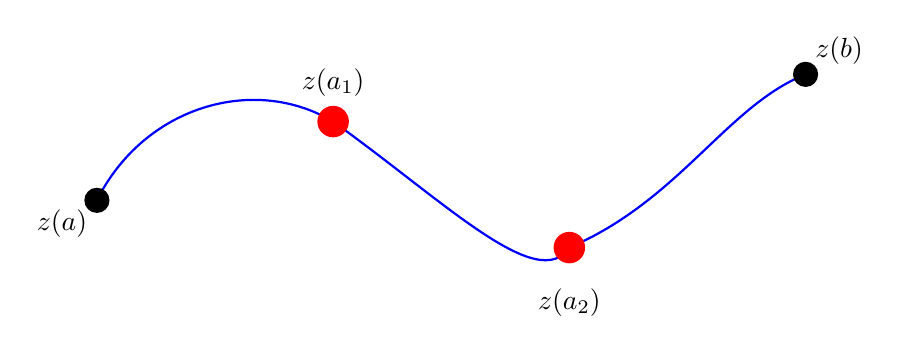
\begin{tikzpicture}[scale=2]
                % First smooth segment
                \draw[thick, blue] (0,0) .. controls (0.3,0.6) and (1,0.8) .. (1.5,0.5);
                % Second smooth segment
                \draw[thick, blue] (1.5,0.5) .. controls (2.2,0) and (2.8,-0.6) .. (3,-0.3);
                % Third smooth segment
                \draw[thick, blue] (3,-0.3) .. controls (3.7,0) and (4,0.6) .. (4.5,0.8);
                
                % Mark the corners (non-smooth points)
                \fill[red] (1.5,0.5) circle (0.1);
                \fill[red] (3,-0.3) circle (0.1);
                
                % Mark start and end
                \fill[black] (0,0) circle (0.08);
                \fill[black] (4.5,0.8) circle (0.08);
                
                % Labels
                \node[below left] at (0,0) {$z(a)$};
                \node[above] at (1.5,0.6) {$z(a_1)$};
                \node[below] at (3,-0.5) {$z(a_2)$};
                \node[above right] at (4.5,0.8) {$z(b)$};
            \end{tikzpicture}
        \end{center}
        The curve consists of smooth segments joined at corner points (marked in red) where the derivative is discontinuous.
    \end{eg}
\begin{defn}
    The family of all equivalent parameterization determines a curve (oriented) $\gamma \subset \C, \gamma = z([a,b])$. \\
    $z(a)$ is the starting point and $z(b)$ is the endpoint of $\gamma.$ $\gamma^{-1}=\gamma$ with reversed orientation
\end{defn}
\begin{defn}
    $\gamma$ is closed if $z(a)=z(b)$ and simple if $z(t_1)\neq z(t_2)$ for all $t_1\neq t_2$. 
\end{defn}
\begin{eg}
    $z(T)=re^{-it}, t\in [0,2\pi]$\\
\end{eg}
\begin{defn}
    A curve has positive orientation if interior is on the left or counterclockwise.
\end{defn}
\begin{defn}
    Give a smooth curve $\gamma \subset \C$ (with parameterization $z:[a,b]\to\C$) with $f:\gamma \to \C$ continuous.\\
    We set 
    \[
    \int_\gamma f=\int_\gamma f(z)dz = \int_{a}^bf(z(t))z'(t)dt
    .\] 
    Since $f(z(t))z'(t)\in \C$ we split the integral into \[
    \int_a^b\Re(...)dt+i\int_a^b\Im(...)dt
    .\]  
\end{defn}
\begin{rmk}
    This is well defined as the right hand side does not depend on the choice of the parametrization. 
\end{rmk}
\begin{defn}
    For a piece-wise smooth curve, we define \[
    \int_\gamma f=\sum_{j=0}^{k-1}\int_{a_j}^{a_{j+1}}f(z(t))z'(t)dt
    .\] 
\end{defn}
\begin{defn}
    We define \[
    |\gamma|= \text{length}(\gamma)=\int_{a}^{b}|z'(t)|dt
    .\] 
\end{defn}
\begin{thm}
    Some very basic properties:
    \begin{enumerate}
        \item Linearity \[
        \int_\gamma (\alpha f+ \beta g)=\alpha \int_\gamma f +\beta \int_\gamma g
        .\] 
        \item \[
        \int_{\gamma^{-1}}f=-\int_{\gamma}f
        .\] 
        \item \[
        \left |\int_\gamma f\right |\leq  \left( \sup_\gamma |f| \right)|\gamma|
        .\] 
    \end{enumerate}
\end{thm}
\begin{defn}
    The primitive of $f:\Omega\to \C$ with open $\Omega\subset \C$ is any $F:\Omega\to \C$ holomorphic such that $F'=f$ on $\Omega$
\end{defn}
\begin{thm}
    The Fundamental Theorem of Calculus\\
    For $f$ with primitive $F$ on $\Omega$, $\gamma\subset \C$ curve from $w_1\to w_2$ we have \[
    \int_\gamma f=F(w_2)-F(w_1)
    .\] 
    \begin{proof}
        We can write \[
        \int_\gamma f=\int_a^bf(z(t))z'(t)dt=\int_a^b \frac{d}{dt}(F(z(t)))dt=F(z(b))-F(z(a))
        .\] 
    \end{proof}
\end{thm}
\begin{cor}
    If $\gamma$ is closed then \[
    \int_\gamma f=0
    .\] 
\end{cor}
\begin{cor}
    If $f$ is holomorphic on $\Omega$ with $f'=0$ on $\Omega$ then $f$ is constant.
    \begin{proof}
        Fix $z_0\in \Omega,$ for $z\in \Omega$, take $\gamma:z_0\to z$ then \[
        0=\int_\gamma f'=f(z)-f(z_0)
        .\] 
    \end{proof}
\end{cor}
\begin{eg}
    Let $z(t)=e^{it}$
    \[
    \int_{\partial D}{ \frac{1}{z}}dz=\int_0^{2\pi}\frac{1}{e^{it}}ie^{it}dt=2\pi i \neq 0
    .\] 
    So $\frac{1}{z}$ does not admit a primitive. 
\end{eg}
\newpage
\section{Jan 23}
\textbf{Glossary of Elementary Functions}
\begin{enumerate}
    \item Polynomials: $P(z)=a_0+a_1z+\cdots+a_nz^n$ for $a_i\in \C$ and is entirely holomorphic in $\C$, $a_n\neq 0 $ and $n=\deg P$
    \item Rational: $R(z)=\frac{P(z)}{Q(z)}$ where $P,Q$ are polynomials with no common factors. The zeros of $Q$ are called poles and their order is called the order of a given pole.
    \item Exponential: $e^z=\sum_{n=0}^\infty \frac{z^n}{n!}$
\end{enumerate}
\begin{lem}
    Let $P(z)$ be a complex polynomial of positive degree $n$, if $|P(z)|$ has a local minimum at $z_0$ then $P(z_0)=0$.
    \begin{proof}
        WLOG $z_0=0$ as we can translate $Q(z)=P(z-z_0)$. \\AFSOC $P(0)\neq 0$ and WLOG $P(0)=1$ by $\frac{P}{P(0)}$. We can write $P(z)=1+a_kz^k+\cdots+a_z^n$ with $a_k,a_n\neq 0$. \\
        Consider $z_\delta = \delta e^{i\theta}.$ For all $\delta>0$ sufficiently small: 
        \[
        \left | a_{k+1}z_\delta + \cdots + a_nz_\delta^{n-k}\right |<\frac{|a_k|}{2}
        .\]  
        Then \[
        |P(z)|\leq \left | 1+a_kz_\delta^k\right | + \left |a_{k+1}z_\delta^{k+1}+\cdots+a_nz_\delta^n\right |< \left | 1+a_kz_\delta^k\right |+\left |z_\delta^k\right | \frac{|a_k|}{2}
        .\]
        Now we can choose $\delta$ such that $a_kz_\delta^k<0$ and real. 
        \[
        \left | 1+a_kz_\delta^k\right |+\left |z_\delta^k\right | \frac{|a_k|}{2}=1+a_kz_\delta^k-\frac{1}{2}a_kz_\delta^k=1+\frac{1}{2}a_kz_\delta^k<1
        .\] 
    \end{proof}
\end{lem}
\begin{thm}
    Fundamental Theorem of Algebra:
    \begin{proof}
        $|P(z)|\to +\infty$ as $|z|\to+\infty$ therefore $\exists R$ such that $\forall |z|>R$, $|P(z)|>|P(0)|$ thus $\inf_{z\in \C}|P(z)|=\inf_{z\in D_R}|P(z)|$ and such a value is attained somewhere at $z_0$ then by lemma 5.1 we're done. 
    \end{proof}
\end{thm}
\begin{lem}
    $P(z)=a_n(z-z_1)\cdots(z-z_n)$ where $z_1,...,z_n$ are roots of $P$.\\ The order of a zero $z_j$ is its multiplicity, the number of times it appears in the sequence. If $z_j$ is of the order $k_j$, \[
    P(z)=\underbrace{Q(z)}_{\mathclap{\text{non-vanishing}}}(z-z_j)^{k_j}
    .\] 
    A zero $z_0$ is of order $k_0$ if and only if $P(z_0)=P'(z_0)=...=P^{(k_0-1)}(z_0)=0$ and $P^{(k_0)}(z_0)\neq 0$
\end{lem}
\begin{thm}
    (Gauss-Lucas) The roots of $P'$ lies in the convex hull of the roots of $P$. In particular, if $P$ is real rooted then so is $P'$. 
\end{thm}
\begin{thm}
    If $R$ a rational function then $R'$ has the same roots as $R$ with order greater by $1$. 
\end{thm}
\begin{thm}
    The following are true
    \begin{enumerate}
        \item $ \left(  e^z \right)'=e^z$
        \item $e^{w+z}=e^we^z$
        \item $\overline{e^z}=e^{\overline{z}}$
        \item $|e^{iy}|=1$ and $|e^{x+iy}|=e^x$
        \item $\sin(z)=\frac{e^{iz}-e^{-iz}}{2i}$ and $\cos(z)=\frac{e^{iz}+e^{-iz}}{2}$
    \end{enumerate}
\end{thm}
\section{Jan 26}
\begin{thm}
    Cauchy Theorem: If $f:\Omega\to \C$ is holomorphic on $\Omega$ and $\gamma$ is a closed curve in $\Omega$ then \[
    \int_\gamma f=0
    .\] 

\end{thm}
\begin{thm}
    Goursat's Theorem: If $f:\Omega\to \C$ is holomorphic and $\Omega$ is open, then $\forall \triangle \subset \Omega$ we have \[
    \int_{\partial \triangle} f=0
    .\] 
    \begin{center}
        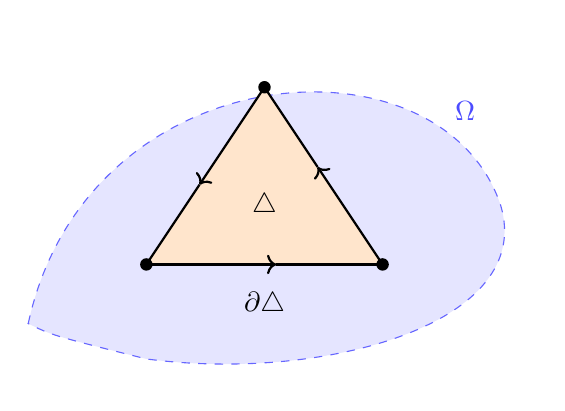
\begin{tikzpicture}[scale=1.5]
            % Draw the open set Omega as a shaded region
            \fill[blue!10] (-0.5,-0.5) .. controls (0,1.8) and (3,2) .. (3.5,0.5) 
                .. controls (3.8,-0.5) and (2,-1) .. (0.5,-0.8) 
                .. controls (-0.3,-0.6) .. cycle;
            \draw[dashed, blue!60] (-0.5,-0.5) .. controls (0,1.8) and (3,2) .. (3.5,0.5) 
                .. controls (3.8,-0.5) and (2,-1) .. (0.5,-0.8) 
                .. controls (-0.3,-0.6) .. cycle;
            \node[blue!70] at (3.2,1.3) {$\Omega$};
            
            % Draw the triangle
            \coordinate (A) at (0.5,0);
            \coordinate (B) at (2.5,0);
            \coordinate (C) at (1.5,1.5);
            
            % Fill triangle
            \fill[orange!20] (A) -- (B) -- (C) -- cycle;
            
            % Draw triangle edges with arrows (counterclockwise orientation)
            \draw[thick, ->] (A) -- ($(A)!0.55!(B)$);
            \draw[thick] ($(A)!0.55!(B)$) -- (B);
            \draw[thick, ->] (B) -- ($(B)!0.55!(C)$);
            \draw[thick] ($(B)!0.55!(C)$) -- (C);
            \draw[thick, ->] (C) -- ($(C)!0.55!(A)$);
            \draw[thick] ($(C)!0.55!(A)$) -- (A);
            
            % Label vertices
            \fill (A) circle (1.5pt);
            \fill (B) circle (1.5pt);
            \fill (C) circle (1.5pt);
            
            % Label the triangle
            \node at (1.5,0.5) {$\triangle$};
            
            % Label the boundary
            \node[below] at (1.5,-0.15) {$\partial \triangle$};
        \end{tikzpicture}
    \end{center}
    The integral around the positively oriented (counterclockwise) boundary of any triangle $\triangle \subset \Omega$ vanishes.
\end{thm}
\begin{proof}
    Let $\triangle=\triangle^{(0)}$ and partition into four triangles by connecting the midpoints of the sides:
    \[
    \triangle^{(0)}=\triangle_1^{(1)}\cup \triangle_2^{(1)} \cup \triangle_3^{(1)} \cup \triangle_4^{(1)}
    .\]
    \begin{center}
        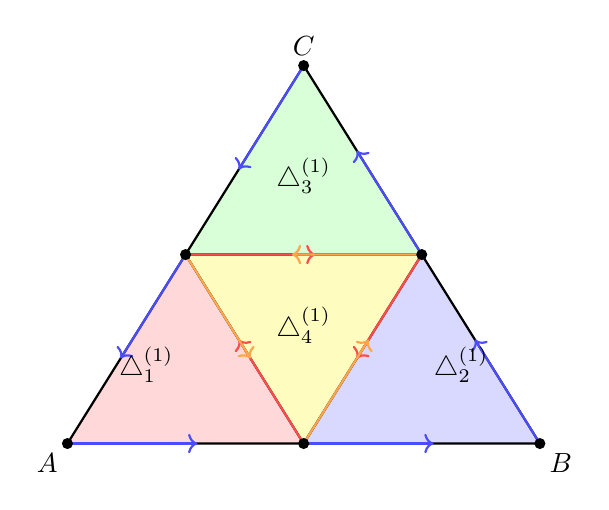
\begin{tikzpicture}[scale=2]
            % Original triangle vertices
            \coordinate (A) at (0,0);
            \coordinate (B) at (3,0);
            \coordinate (C) at (1.5,2.4);
            
            % Midpoints
            \coordinate (MAB) at ($(A)!0.5!(B)$);
            \coordinate (MBC) at ($(B)!0.5!(C)$);
            \coordinate (MCA) at ($(C)!0.5!(A)$);
            
            % Fill the four triangles with different colors
            \fill[red!15] (A) -- (MAB) -- (MCA) -- cycle;
            \fill[blue!15] (MAB) -- (B) -- (MBC) -- cycle;
            \fill[green!15] (MCA) -- (MBC) -- (C) -- cycle;
            \fill[yellow!25] (MAB) -- (MBC) -- (MCA) -- cycle;
            
            % Draw outer triangle
            \draw[thick] (A) -- (B) -- (C) -- cycle;
            
            % Draw inner edges (midpoint connections)
            \draw[thick] (MAB) -- (MBC) -- (MCA) -- cycle;
            
            % Arrows on outer boundary (counterclockwise)
            \draw[thick, ->, blue!70] (A) -- ($(A)!0.55!(MAB)$);
            \draw[thick, ->, blue!70] (MAB) -- ($(MAB)!0.55!(B)$);
            \draw[thick, ->, blue!70] (B) -- ($(B)!0.55!(MBC)$);
            \draw[thick, ->, blue!70] (MBC) -- ($(MBC)!0.55!(C)$);
            \draw[thick, ->, blue!70] (C) -- ($(C)!0.55!(MCA)$);
            \draw[thick, ->, blue!70] (MCA) -- ($(MCA)!0.55!(A)$);
            
            % Arrows on inner edges showing cancellation (both directions)
            \draw[thick, ->, red!70] (MAB) -- ($(MAB)!0.55!(MCA)$);
            \draw[thick, ->, orange!70] (MCA) -- ($(MCA)!0.55!(MAB)$);
            \draw[thick, ->, red!70] (MBC) -- ($(MBC)!0.55!(MAB)$);
            \draw[thick, ->, orange!70] (MAB) -- ($(MAB)!0.55!(MBC)$);
            \draw[thick, ->, red!70] (MCA) -- ($(MCA)!0.55!(MBC)$);
            \draw[thick, ->, orange!70] (MBC) -- ($(MBC)!0.55!(MCA)$);
            
            % Labels for vertices
            \fill (A) circle (1pt) node[below left] {$A$};
            \fill (B) circle (1pt) node[below right] {$B$};
            \fill (C) circle (1pt) node[above] {$C$};
            
            % Labels for midpoints
            \fill (MAB) circle (1pt);
            \fill (MBC) circle (1pt);
            \fill (MCA) circle (1pt);
            
            % Labels for the four triangles
            \node at (0.5,0.5) {$\triangle_1^{(1)}$};
            \node at (2.5,0.5) {$\triangle_2^{(1)}$};
            \node at (1.5,1.7) {$\triangle_3^{(1)}$};
            \node at (1.5,0.75) {$\triangle_4^{(1)}$};
        \end{tikzpicture}
    \end{center}
    When we integrate along each sub-triangle with positive orientation, the interior edges cancel (traversed in opposite directions, shown with opposing arrows): \[
    \int_{\partial \triangle^{(0)}} f= \sum_{j=1}^4 \int_{\partial \triangle_j^{(1)}} f
    .\]     
    By the triangle inequality 
    \[
        \left | \int_{\partial \triangle^{(0)}}f \right |\leq \sum_{j=1}^4 \left | \int_{\partial \triangle_j^{(1)}}f \right | \leq 4 \max_{j=1,2,3,4} \left | \int_{\partial \triangle_j^{(1)}}f \right |
    .\] 
    Thus there exists $j_0\in\{1,2,3,4\}$ such that\[
     \left | \int_{\partial \triangle^{(0)}}f \right |\leq 4\left | \int_{\partial \triangle_{j_0}^{(1)}}f \right |
    .\]
    Set $\triangle^{(1)}=\triangle_{j_0}^{(1)}$. Repeating this subdivision process, we obtain a nested sequence of triangles 
    \[
    \triangle^{(0)}\supset \triangle^{(1)}\supset \triangle^{(2)}\supset \cdots
    \]
    such that 
    \[
        \left | \int_{\partial \triangle^{(0)}}f \right |\leq 4^n \left | \int_{\partial \triangle^{(n)}}f \right |
    .\]
    Note that $\diam(\triangle^{(n)})=2^{-n}\diam(\triangle^{(0)})$ and $|\partial \triangle^{(n)}|=2^{-n}|\partial \triangle^{(0)}|$.\\
    Since the triangles are nested compact sets with diameters shrinking to zero, by Cantor's intersection theorem:
    \[
    \bigcap_{n=0}^\infty \triangle^{(n)}=\{z_0\}
    \]
    for some $z_0\in \triangle^{(0)}\subset \Omega$.
    Since $f$ is holomorphic at $z_0$, we can write \[
    f(z)=f(z_0)+f'(z_0)(z-z_0)+\psi(z)(z-z_0) 
    \] 
    where $\psi(z)\to 0$ as $z\to z_0$.\\
    Since $f(z_0)$ and $f'(z_0)(z-z_0)$ have primitives ($f(z_0)z$ and $\frac{1}{2}f'(z_0)(z-z_0)^2$ respectively), their integrals over the closed curve $\partial \triangle^{(n)}$ vanish. Thus:
    \[
    \int_{\partial \triangle^{(n)}}f(z)dz=\int_{\partial \triangle^{(n)}}\psi(z)(z-z_0)dz
    .\] 
    For $z\in \partial \triangle^{(n)}$, we have $|z-z_0|\leq \diam(\triangle^{(n)})=2^{-n}\diam(\triangle^{(0)})$. \\
    Let $\epsilon_n=\sup_{z\in\partial\triangle^{(n)}}|\psi(z)|$. Since $\psi(z)\to 0$ as $z\to z_0$ and $\triangle^{(n)}\to \{z_0\}$, we have $\epsilon_n\to 0$.\\
    Therefore:
    \begin{align*}
        \left | \int_{\partial \triangle^{(n)}}f(z)dz \right | &\leq \sup_{z\in\partial \triangle^{(n)}}|\psi(z)(z-z_0)| \cdot |\partial \triangle^{(n)}|\\
        &\leq \epsilon_n \cdot 2^{-n}\diam(\triangle^{(0)})\cdot 2^{-n}|\partial \triangle^{(0)}|\\
        &= \epsilon_n \cdot 4^{-n}\diam(\triangle^{(0)})|\partial \triangle^{(0)}|
    \end{align*}
    Combining with our earlier inequality:
    \[
    \left | \int_{\partial \triangle^{(0)}}f \right |\leq 4^n \left | \int_{\partial \triangle^{(n)}}f \right | \leq 4^n \cdot \epsilon_n \cdot 4^{-n}\diam(\triangle^{(0)})|\partial \triangle^{(0)}| = \epsilon_n \cdot \diam(\triangle^{(0)})|\partial \triangle^{(0)}|
    \]
    Since $\epsilon_n\to 0$ as $n\to\infty$ and the right-hand side is independent of $n$ except for $\epsilon_n$, we conclude:
    \[
    \int_{\partial \triangle}f=0
    .\]
\end{proof}
\begin{thm}
    Cauchy's Theorem in a disk: Let $D\subset \C$ be an open disk and $f$ holomorphic on $D$. Then for any closed curve $\gamma$ in $D$ we have \[
    \int_\gamma f=0
    .\] 
    \begin{proof}
        WLOG let $D$ be a disk centered at $0$. Define $F:D\to \C$ by \[
        F(z)=\int_{\gamma_z}f
        \]
        where $\gamma_z$ is the path $0\to \Re(z)\to z$ (horizontal then vertical).
        \begin{center}
            \begin{tikzpicture}[scale=1.2]
                % Draw the disk
                \draw[dashed, blue!50] (0,0) circle (2.2);
                \node[blue!70] at (1.8,1.8) {$D$};
                
                % Axes
                \draw[->] (-2.5,0) -- (2.5,0) node[right] {$\Re$};
                \draw[->] (0,-2.5) -- (0,2.5) node[above] {$\Im$};
                
                % Points
                \coordinate (O) at (0,0);
                \coordinate (X) at (1.5,0);
                \coordinate (Z) at (1.5,1.2);
                
                % Path gamma_z
                \draw[thick, blue, ->] (O) -- (0.8,0);
                \draw[thick, blue] (0.8,0) -- (X);
                \draw[thick, blue, ->] (X) -- (1.5,0.6);
                \draw[thick, blue] (1.5,0.6) -- (Z);
                
                % Labels
                \fill (O) circle (1.5pt) node[below left] {$0$};
                \fill (X) circle (1.5pt) node[below] {$\Re(z)$};
                \fill (Z) circle (1.5pt) node[above right] {$z$};
                
                % Path label
                \node[blue] at (0.75,0.3) {$\gamma_z$};
            \end{tikzpicture}
        \end{center}
        We claim $F$ is a primitive for $f$, i.e., $F'(z)=f(z)$.\\[6pt]
        \textbf{Case 1:} $h\in \R$ (horizontal increment).\\
        The path $\gamma_{z+h}$ goes $0\to \Re(z)+h\to z+h$. Observe that:
        \[
        F(z+h)-F(z)= \int_{\gamma_{z+h}}f-\int_{\gamma_z}f
        .\]
        \begin{center}
            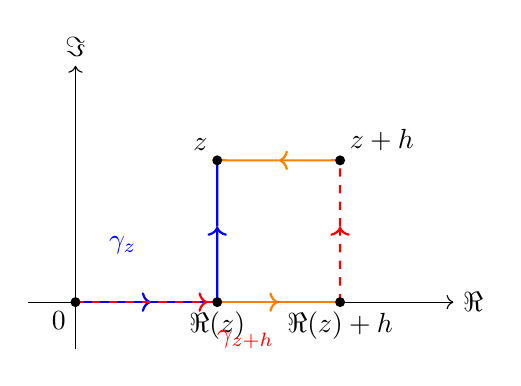
\begin{tikzpicture}[scale=1.2]
                % Axes
                \draw[->] (-0.5,0) -- (4,0) node[right] {$\Re$};
                \draw[->] (0,-0.5) -- (0,2.5) node[above] {$\Im$};
                
                % Points
                \coordinate (O) at (0,0);
                \coordinate (X) at (1.5,0);
                \coordinate (Xh) at (2.8,0);
                \coordinate (Z) at (1.5,1.5);
                \coordinate (Zh) at (2.8,1.5);
                
                % Path gamma_z (blue)
                \draw[thick, blue, ->] (O) -- (0.8,0);
                \draw[thick, blue] (0.8,0) -- (X);
                \draw[thick, blue, ->] (X) -- (1.5,0.8);
                \draw[thick, blue] (1.5,0.8) -- (Z);
                
                % Path gamma_{z+h} (red, dashed)
                \draw[thick, red, dashed, ->] (O) -- (1.4,0);
                \draw[thick, red, dashed] (1.4,0) -- (Xh);
                \draw[thick, red, dashed, ->] (Xh) -- (2.8,0.8);
                \draw[thick, red, dashed] (2.8,0.8) -- (Zh);
                
                % Rectangle (the key region)
                \draw[thick, orange, ->] (X) -- (2.15,0);
                \draw[thick, orange] (2.15,0) -- (Xh);
                \draw[thick, orange, ->] (Zh) -- (2.15,1.5);
                \draw[thick, orange] (2.15,1.5) -- (Z);
                
                % Labels
                \fill (O) circle (1.5pt) node[below left] {$0$};
                \fill (X) circle (1.5pt) node[below] {$\Re(z)$};
                \fill (Xh) circle (1.5pt) node[below] {$\Re(z)+h$};
                \fill (Z) circle (1.5pt) node[above left] {$z$};
                \fill (Zh) circle (1.5pt) node[above right] {$z+h$};
                
                % Path labels
                \node[blue] at (0.5,0.6) {$\gamma_z$};
                \node[red] at (1.8,-0.4) {$\gamma_{z+h}$};
            \end{tikzpicture}
        \end{center}
        The difference of paths can be decomposed using Goursat's theorem. The integral over the rectangle with vertices $\Re(z), \Re(z)+h, z+h, z$ vanishes, so:
        \[
        F(z+h)-F(z)=\int_{\Re(z)}^{\Re(z)+h}f(\zeta)d\zeta + \int_{z}^{z+h}f(\zeta)d\zeta = \int_{z}^{z+h}f(\zeta)d\zeta
        \]
        where the first integral is along the real axis and the second is horizontal at height $\Im(z)$. By the rectangle lemma, these combine to give just the horizontal segment from $z$ to $z+h$:
        \[
        \frac{F(z+h)-F(z)}{h}=\frac{1}{h}\int_z^{z+h}f(\zeta)d\zeta \to f(z) \text{ as } h\to 0
        .\]
        \textbf{Case 2:} $h=ik$ with $k\in \R$ (vertical increment).\\
        Similarly, $\gamma_{z+ik}$ goes $0\to \Re(z)\to z+ik$. The paths $\gamma_z$ and $\gamma_{z+ik}$ share the horizontal segment $0\to \Re(z)$, so:
        \[
        F(z+ik)-F(z)=\int_z^{z+ik}f(\zeta)d\zeta
        .\]
        \begin{center}
            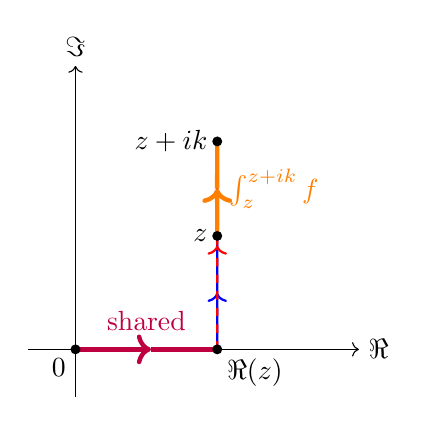
\begin{tikzpicture}[scale=1.2]
                % Axes
                \draw[->] (-0.5,0) -- (3,0) node[right] {$\Re$};
                \draw[->] (0,-0.5) -- (0,3) node[above] {$\Im$};
                
                % Points
                \coordinate (O) at (0,0);
                \coordinate (X) at (1.5,0);
                \coordinate (Z) at (1.5,1.2);
                \coordinate (Zik) at (1.5,2.2);
                
                % Shared horizontal path (purple)
                \draw[ultra thick, purple, ->] (O) -- (0.8,0);
                \draw[ultra thick, purple] (0.8,0) -- (X);
                
                % Path to z (blue)
                \draw[thick, blue, ->] (X) -- (1.5,0.6);
                \draw[thick, blue] (1.5,0.6) -- (Z);
                
                % Path to z+ik (red, dashed)
                \draw[thick, red, dashed, ->] (X) -- (1.5,1.1);
                \draw[thick, red, dashed] (1.5,1.1) -- (Zik);
                
                % The difference segment (orange)
                \draw[ultra thick, orange, ->] (Z) -- (1.5,1.7);
                \draw[ultra thick, orange] (1.5,1.7) -- (Zik);
                
                % Labels
                \fill (O) circle (1.5pt) node[below left] {$0$};
                \fill (X) circle (1.5pt) node[below right] {$\Re(z)$};
                \fill (Z) circle (1.5pt) node[left] {$z$};
                \fill (Zik) circle (1.5pt) node[left] {$z+ik$};
                
                % Path labels
                \node[purple] at (0.75,0.3) {shared};
                \node[orange] at (2.1,1.7) {$\int_z^{z+ik}f$};
            \end{tikzpicture}
        \end{center}
        Thus:
        \[
        \frac{F(z+ik)-F(z)}{ik}=\frac{1}{ik}\int_z^{z+ik}f(\zeta)d\zeta \to f(z) \text{ as } k\to 0
        .\]
        \textbf{General $h$:} For arbitrary $h=h_1+ih_2$, we write:
        \[
        \frac{F(z+h)-F(z)}{h}=\frac{F(z+h)-F(z+h_1)}{h}+\frac{F(z+h_1)-F(z)}{h}
        .\]
        Using the above cases and the continuity of $f$, both terms converge appropriately, giving $F'(z)=f(z)$.\\[6pt]
        Since $f$ has a primitive $F$ on $D$, by the Fundamental Theorem of Calculus, for any closed curve $\gamma$ in $D$:
        \[
        \int_\gamma f = F(z(b))-F(z(a))=0
        .\]
    \end{proof}
\end{thm}
\newpage
\section{Jan 28}
\begin{eg}
    \[
    \frac{1}{\sqrt{\pi}}\int_{-\infty}^{\infty}e^{-x^2}dx=1 \iff \int_{-\infty}^{\infty}e^{-\pi x^2}dx=1
    .\] 
    \begin{proof}
        First, note that by substitution $u=\sqrt{\pi}x$, we have:
        \[
        \int_{-\infty}^{\infty}e^{-\pi x^2}dx = \frac{1}{\sqrt{\pi}}\int_{-\infty}^{\infty}e^{-u^2}du
        .\]
        So the equivalence follows if we can show $\int_{-\infty}^{\infty}e^{-\pi x^2}dx=1$.\\\\
        Consider the function $f(z)=e^{-\pi z^2}$, which is entire (holomorphic everywhere). For fixed $y\in \R$, consider the rectangular contour $\Gamma_R$ with vertices at $-R, R, R+iy, -R+iy$ (traversed counterclockwise). 
        \begin{center}
            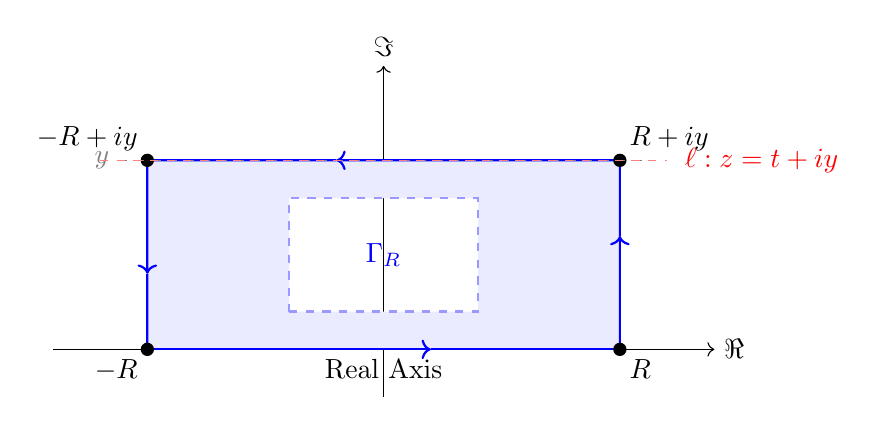
\begin{tikzpicture}[scale=1.2]
                % Axes
                \draw[->] (-3.5,0) -- (3.5,0) node[right] {$\Re$};
                \draw[->] (0,-0.5) -- (0,3) node[above] {$\Im$};
                
                % Real axis label
                \node[below] at (0,0) {Real Axis};
                
                % Rectangle vertices
                \coordinate (A) at (-2.5,0);
                \coordinate (B) at (2.5,0);
                \coordinate (C) at (2.5,2);
                \coordinate (D) at (-2.5,2);
                
                % Inner rectangle (cut-out center)
                \coordinate (Ainner) at (-1,0.4);
                \coordinate (Binner) at (1,0.4);
                \coordinate (Cinner) at (1,1.6);
                \coordinate (Dinner) at (-1,1.6);
                
                % Create donut shape: fill outer rectangle but cut out center
                \fill[blue!8, even odd rule] (A) -- (B) -- (C) -- (D) -- cycle 
                    (Ainner) -- (Binner) -- (Cinner) -- (Dinner) -- cycle;
                
                % Draw the outer rectangle boundary with arrows showing counterclockwise orientation
                \draw[thick, blue, ->] (A) -- ($(A)!0.6!(B)$);
                \draw[thick, blue] ($(A)!0.6!(B)$) -- (B);
                \draw[thick, blue, ->] (B) -- ($(B)!0.6!(C)$);
                \draw[thick, blue] ($(B)!0.6!(C)$) -- (C);
                \draw[thick, blue, ->] (C) -- ($(C)!0.6!(D)$);
                \draw[thick, blue] ($(C)!0.6!(D)$) -- (D);
                \draw[thick, blue, ->] (D) -- ($(D)!0.6!(A)$);
                \draw[thick, blue] ($(D)!0.6!(A)$) -- (A);
                
                % Draw inner rectangle boundary (showing the cut-out)
                \draw[thick, blue!40, dashed] (Ainner) -- (Binner) -- (Cinner) -- (Dinner) -- cycle;
                
                % Mark vertices
                \fill (A) circle (2pt) node[below left] {$-R$};
                \fill (B) circle (2pt) node[below right] {$R$};
                \fill (C) circle (2pt) node[above right] {$R+iy$};
                \fill (D) circle (2pt) node[above left] {$-R+iy$};
                
                % Label the contour
                \node[blue] at (0,1) {$\Gamma_R$};
                
                % Dashed line showing y
                \draw[dashed, gray] (-2.8,2) -- (2.8,2);
                \node[left, gray] at (-2.8,2) {$y$};
                
                % Label showing the horizontal line
                \draw[dashed, red!50] (-3,2) -- (3,2);
                \node[red] at (4,2) {$\ell: z=t+iy$};
            \end{tikzpicture}
        \end{center}
        By Cauchy's theorem:
        \[
        \int_{\Gamma_R}e^{-\pi z^2}dz=0
        .\]
        Parameterizing the four sides:
        \begin{align*}
            \int_{\Gamma_R}e^{-\pi z^2}dz &= \int_{-R}^{R}e^{-\pi t^2}dt + \int_{0}^{y}e^{-\pi(R+it)^2}i\,dt \\
            &\quad + \int_{R}^{-R}e^{-\pi(t+iy)^2}dt + \int_{y}^{0}e^{-\pi(-R+it)^2}i\,dt
        \end{align*}
        We now bound the integrals over the vertical segments. For the right vertical segment, parameterize $z=R+it$ with $t\in[0,y]$ (assuming $y>0$; the case $y<0$ is similar). We have:
        \[
        (R+it)^2 = R^2 + 2iRt - t^2 = (R^2-t^2) + 2iRt
        \]
        so
        \[
        e^{-\pi(R+it)^2} = e^{-\pi(R^2-t^2)} \cdot e^{-2\pi iRt}
        .\]
        Since $|e^{-2\pi iRt}| = 1$ for all real $R$ and $t$, we have:
        \[
        |e^{-\pi(R+it)^2}| = e^{-\pi(R^2-t^2)} \cdot |e^{-2\pi iRt}| = e^{-\pi(R^2-t^2)} \cdot 1 = e^{-\pi(R^2-t^2)}
        .\]
        For $t\in[0,y]$, we have $t^2 \leq y^2$, so $R^2-t^2 \geq R^2-y^2$. Therefore:
        \[
        |e^{-\pi(R+it)^2}| \leq e^{-\pi(R^2-y^2)} = e^{-\pi R^2}e^{\pi y^2}
        .\]
        By the ML-inequality, the length of the path is $|y|$, so:
        \[
        \left|\int_{0}^{y}e^{-\pi(R+it)^2}i\,dt\right| \leq |y| \cdot e^{-\pi R^2}e^{\pi y^2} = |y|e^{\pi y^2}e^{-\pi R^2}
        .\]
        Similarly, for the left vertical segment with $z=-R+it$ where $t\in[y,0]$:
        \[
        (-R+it)^2 = R^2 - 2iRt - t^2 = (R^2-t^2) - 2iRt
        \]
        so
        \[
        e^{-\pi(-R+it)^2} = e^{-\pi(R^2-t^2)} \cdot e^{2\pi iRt}
        .\]
        Since $|e^{2\pi iRt}| = 1$ for all real $R$ and $t$, we have:
        \[
        |e^{-\pi(-R+it)^2}| = e^{-\pi(R^2-t^2)} \cdot |e^{2\pi iRt}| = e^{-\pi(R^2-t^2)} \cdot 1 = e^{-\pi(R^2-t^2)}
        .\]
        For $t\in[y,0]$ (or equivalently $t\in[0,y]$ if we reverse the parameterization), we have $t^2 \leq y^2$, so:
        \[
        |e^{-\pi(-R+it)^2}| \leq e^{-\pi(R^2-y^2)} = e^{-\pi R^2}e^{\pi y^2}
        .\]
        Therefore:
        \[
        \left|\int_{y}^{0}e^{-\pi(-R+it)^2}i\,dt\right| \leq |y| \cdot e^{-\pi R^2}e^{\pi y^2} = |y|e^{\pi y^2}e^{-\pi R^2}
        .\]
        Both vertical integrals are bounded by $C e^{-\pi R^2}$ for some constant $C$ depending on $y$ but independent of $R$. Since $e^{-\pi R^2} \to 0$ as $R\to\infty$, we conclude that:
        \[
        \lim_{R\to\infty}\int_{0}^{y}e^{-\pi(R+it)^2}i\,dt = 0 \quad \text{and} \quad \lim_{R\to\infty}\int_{y}^{0}e^{-\pi(-R+it)^2}i\,dt = 0
        .\]
        Therefore, taking the limit as $R\to\infty$:
        \[
        \int_{-\infty}^{\infty}e^{-\pi t^2}dt = \int_{-\infty}^{\infty}e^{-\pi(t+iy)^2}dt
        .\]
        Expanding $e^{-\pi(t+iy)^2}=e^{-\pi(t^2+2ity-y^2)}=e^{-\pi t^2}e^{-2\pi ity}e^{\pi y^2}$, we get:
        \[
        \int_{-\infty}^{\infty}e^{-\pi t^2}dt = e^{\pi y^2}\int_{-\infty}^{\infty}e^{-\pi t^2}e^{-2\pi ity}dt
        .\]
        In particular, taking $y=0$ gives the standard Gaussian integral. The standard result is $\int_{-\infty}^{\infty}e^{-\pi x^2}dx=1$, which completes the proof.
    \end{proof}
\end{eg}
\begin{eg}
    \[
    \int_0^{\infty}\frac{1-\cos(x)}{x^2}dx=\frac{\pi}{2}
    .\] 
    \begin{proof}
        Consider the holomorphic function $f(z)=\frac{1-e^{iz}}{z^2}$ on $\C\setminus \{0\}$. Fix $\epsilon, R$ and consider the contour $\Gamma$ which is disk with radius $R$ and a small disk with radius $\epsilon$ centered at the origin.
    \begin{center}
    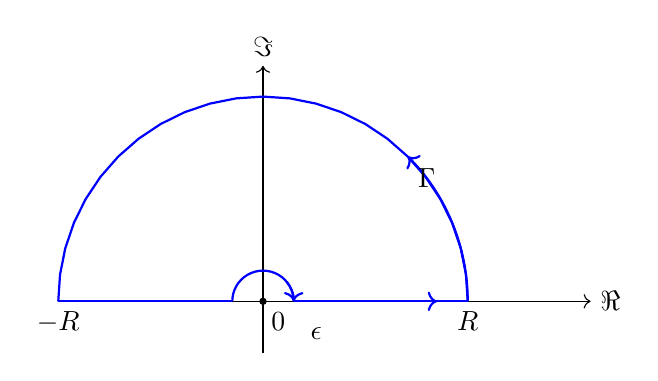
\begin{tikzpicture}[scale=1.3]
        % Draw the axes
        \draw[->] (-0.5,0) -- (3.2,0) node[right] {$\Re$};
        \draw[->] (0,-0.5) -- (0,2.3) node[above] {$\Im$};

        % Draw the large semicircle
        \draw[thick,blue,domain=0:180] plot ({2*cos(\x)}, {2*sin(\x)});

        % Draw the small indentation
        \draw[thick,blue,domain=0:180] plot ({0.3*cos(\x)}, {0.3*sin(\x)});

        % Draw the lines along the real axis outside the indentation
        \draw[thick,blue] (0.3,0) -- (2,0);
        \draw[thick,blue] (-2,0) -- (-0.3,0);

        % Draw arrows to indicate the direction of the contour
        \draw[thick,->,blue] (1,0) -- (1.7,0); % Rightward along real axis
        \draw[thick,->,blue] ({0.3*cos(40)},{0.3*sin(40)}) arc (40:0:0.3); % Small arc (reversed direction)
        \draw[thick,->,blue] (2,{0.001}) arc (0:45:2); % Large arc

        % Label the points
        \draw (2,0) node[below] {$R$};
        \draw (-2,0) node[below] {$-R$};
        \draw (0.37,-0.16) node[below right] {$\epsilon$};
        \node at (1.6,1.2) {$\Gamma$};
        % Mark origin
        \filldraw (0,0) circle (0.03);
        \node at (0.15,-0.2) {$0$};
    \end{tikzpicture}
    \end{center}
    We can express $e^{iz}\approx 1+iz+g(z)$ where $g(z)=e^{iz}-1-iz$ so \begin{align*}
        \int_{\gamma_\epsilon}f(z)dz&=\int_{\gamma_\epsilon}\frac{1-(1+iz+g(z))}{z^2}dz \\
        &=\int_{\gamma_\epsilon}\frac{-g(z)}{z^2}dz +\int_{\gamma_\epsilon}\frac{-i}{z}dz
    \end{align*}  
    We can evaluate each part as \[
    \int_{\gamma_\epsilon} \frac{dz}{z}=-\int_{0}^{\pi}\frac{ie^{it}}{e^{it}}dt=-\pi i
    .\] 
    \[
    \int_{\gamma_\epsilon} \frac{g(z)}{z^2}dz\to 0 \text{ as } \epsilon\to 0
    .\] 
    \end{proof}
\end{eg}
\newpage
\section{Jan 30}
\begin{thm}
    Cauchy's Integral Formula: Let $\Omega$ be open $f:\Omega\to \C$ be holomorphic. Let $\overline{D}$ be open in $\Omega$ be a disk then \[
    f(z)=\frac{1}{2\pi i}\int_{\partial D}\frac{f(\zeta)}{\zeta-z}d\zeta
    .\] 
    \begin{proof}
        Fix $z\in D_1$, let $\gamma_{\epsilon, \delta}$ be a key-hole contour but we omit $z.$ Then \[
        \int_{\gamma_{\epsilon, \delta}}\frac{f(\zeta)}{\zeta - z}d\zeta=0
        .\] 
        Fix $\epsilon > 0$ and $\delta \to 0$ we want to show that \[
        \int_{\gamma_{\epsilon, \delta}}\frac{f(\zeta)}{\zeta - z}d\zeta\to \int_{\partial D} - \int_{C_\epsilon}
        .\] 
        For \[
        \int_{C_\epsilon}\frac{f(\zeta)}{\zeta - z}d\zeta = \int_{C_\epsilon}\frac{f(\zeta)-f(z)}{\zeta - z}d\zeta + f(z)\int_{C_\epsilon}\frac{d\zeta}{\zeta - z}
        .\] 
        The first term is bounded as holomorphic so as $\epsilon\to 0$, it goes to $0.$ The second part integrates to $f(z) \cdot 2\pi i.$ 
    \end{proof}
    \end{thm}
\begin{thm}
    Regularity: Holomorphic implies Analytic. \\
    Let $f:\Omega\to \C$ be holomorphic, $\overline{D}=\overline{D}_r(z_0)\subset \Omega$ then $f$ is analytic at $z_0$ i.e \[
    f(z)=\sum_{n=0}^\infty a_n(z-z_0)^n
    .\] 
    \begin{proof}
        We know \[
        f(z)=\frac{1}{2\pi i}\int_{\partial D}\frac{f(\zeta)}{\zeta-z}d\zeta
        .\] 
        We can write \[
        \frac{1}{\zeta-z}=\frac{1}{(\zeta-z_0)+(z_0-z)}=\frac{1}{\zeta - z_0}\cdot \frac{1}{1-\frac{z-z_0}{\zeta - z_0}}=\frac{1}{\zeta-z_0}\sum_{n=0}^\infty \left (\frac{z-z_0}{\zeta-z_0}\right )^n
        .\] 
        Note: $\frac{z-z_0}{\zeta-z_0}<1$. 
        \begin{align*}
            f(z)&=\frac{1}{2\pi i}\int_{\partial D}\frac{f(\zeta)}{\zeta-z_0}\underbrace{\sum_{n=0}^\infty \left (\frac{z-z_0}{\zeta-z_0}\right )^n \frac{f(\zeta)}{\zeta -z}}_{ \text{conv. uniformly on $\partial D$}} d\zeta\\
            &=\frac{1}{2\pi i}\sum_{n=0}^\infty \int_{\partial D}\frac{f(\zeta)}{\zeta-z_0}\left (\frac{z-z_0}{\zeta-z_0}\right )^n d\zeta\\
            &=\sum_{n=0}^{\infty} (z-z_0)^n 
                \underbrace{\left( \frac{1}{2\pi i} \int_{\partial D} \frac{f(\zeta)}{(\zeta-z_0)^{n+1}} d\zeta \right)}_{a_n}
        \end{align*}
        So $a_n=\frac{f^{(n)}(z_0)}{n!}$.
    \end{proof}
\end{thm}
\begin{cor}
    Cauchy's Formula:
    \[
    f^{(n)}(z_0)=\frac{n!}{2\pi i}\int_{\partial D}\frac{f(\zeta)}{(\zeta-z_0)^{n+1}}d\zeta
    .\] 
\end{cor}
\begin{cor}
    Cauchy's Inequality:
    \[
    \left | f^{(n)}(z_0) \right | \leq \frac{n!}{2\pi} \sup_{\zeta\in \partial D} \left | \frac{f(\zeta)}{(\zeta-z_0)^{n+1}} \right |=\frac{n!}{r^n}||f||_\infty\partial D
    .\] 
\end{cor}
\begin{thm}
    Liouville's Theorem: If $f$ entire and bounded then $f$ is constant.
    \begin{proof}
        \[
        |f'(z_0)| \leq \frac{\|f\|_\infty}{r}
        \]
        Since $f$ is bounded and $r$ can be taken arbitrarily large (as $f$ is entire), sending $r \to \infty$ gives $|f'(z_0)| = 0$. Thus, $f$ is constant.
    \end{proof}
\end{thm}
\newpage
\section{Feb 2}
\begin{thm}
    (Rigidity Theorem): Let $\Omega$ be a region and $f:\Omega\to \C$ be holomorphic. If $z_1,z_2,...\in \Omega$ distinct sequence with a limit in $\Omega$. If $f(z_n)=0 \forall n$ then $f=0$ on $\Omega.$
    \begin{proof}
        Say $z_n\to \omega\in \Omega$ and $D=D_r(\omega)\subset \Omega$ be a disk centered at $\omega$ with radius $r$. If $f=0$ on $D$ then by regularity implies \[
        f(z)=\sum_{n\geq 0}a_n(z-\omega)^n \text{ on } D
        .\] 
        Suppose $f\neq 0$ on $D$ then $\exists m$ such that $a_m\neq 0$, let's take the smallest such $m$. Then $f(z)=a_m(z-w)^m(1+g(z))$ where $g(z)\to 0$ as $z\to w.$ For all sufficiency large $k, z_k\in D$ then \[
        0=f(z_k)=a_m(z_k-w)^m(1+g(z_k)) \tag{$a_m\neq 0$ and $z_k-w\neq 0$}
        .\] 
        A contradiction as the RHS is nonzero. To finish $f=0$ on $\Omega$, we use $\mathcal{U}=\text{int} \{z\in \Omega: f(z)=0\}$\\
        We have $\mathcal{U}$ is open, $w\in \mathcal{U}$ so $\mathcal{U}$ is non-empty. Additionally, $\mathcal{U}$ is closed. We have $\Omega\setminus \mathcal{U}$ is open and non-empty so $\exists z_k\in \Omega\setminus \mathcal{U}$ such that $z_k\to \omega'\in \Omega\setminus \mathcal{U}$. Then $f(z_k)\neq 0$ for all $k$ so $f\neq 0$ on $D_r(\omega')$. A contradiction as $D_r(\omega')\subset D$. Thus, $f=0$ on $\Omega$.
    \end{proof}
\end{thm}
\begin{cor}
    $f,g:\underset{region}{\Omega}\to \C$ holomorphic. If $f(z_n)=g(z_n),  \forall z_n\in \Omega$ distinct sequence with a limit in $\Omega$ then $f=g$ on $\Omega.$
\end{cor}
\begin{defn}
    If $\Omega_1\subset \Omega_2,$ are two regions, $f_i:\Omega_i\to \C$ holomorphic for $i=1,2$ such that $f_1=f_2$ on $\Omega_1$ then we say $f_2$ is the analytic continuation of $f_1$ into $\Omega_2.$  
\end{defn}
\begin{thm}
    (Morera's Theorem): If $f:\mathcal{D}\to \C$ continuous such that $\forall \overline{\triangle}\subset \mathcal{D}$ and $\int_{\partial \triangle}f=0$ then $f$ is holomorphic. 
    \begin{proof}
        Repeating the proof of Cauchy's Theorem in a disk, gives that $f$ has a primitive $F=\int_{\gamma_z}f$ in $\mathcal{D}.$ Since $F$ is holomorphic, $F'$ exists but so does $F'',F''',...$ so $f'$ exists. 
    \end{proof}
\end{thm}
\begin{thm}
    If $f_n:\underset{open}{\Omega}\to \C$ holomorphic with $f_n$ converging uniformly to $f$ on every compact $K\subset \Omega$ then $f$ is holomorphic. 
    \begin{proof}
        Use Morera's Theorem. 
    \end{proof}
    \noindent Moreover, if $f_n'$ converges uniformly to $f'$, using $\Omega_s= \{z\in \Omega: \overline{\mathcal{D}}_\delta(z)\subset \Omega\}$. \\
    Claim: $\forall F$ holomorphic in $\Omega,$ $||F'||_{\infty,\Omega_\delta}\leq \frac{1}{\delta}||F||_{\infty, \Omega_\delta}.$ \\
    By Cauchy,s Formula:\[
    |F'(z)|=\left | \frac{1}{2\pi i}\int_{\partial \mathcal{D}_\delta(z)}\frac{F(w)}{(w-z)^2}dw\right |\leq \frac{1}{2\pi}\int_{\partial \mathcal{D}_\delta(z)}\frac{1}{|w-z|^2}||F||_{\infty,\Omega}\leq \frac{1}{2\pi} \frac{2\pi \delta}{\delta^2}||F||_{\infty,\Omega}\leq \frac{1}{\delta}||F||_{\infty,\Omega}
    .\] 
\end{thm}
\newpage
\section{Feb 4}
\begin{thm}
    Let $F:\Omega\times [0,1]\to \C$ satisfy 
    \begin{enumerate}
        \item $\forall \triangle\in [0,1]$, $z\mapsto F(z,\triangle)$ is holomorphic    
        \item $F$ is continuous on $\Omega\times [0,1]$
    \end{enumerate}
    Then $z\mapsto \int_0^1 F(z,\triangle)d\triangle$ is holomorphic on $\Omega$. 
\end{thm}
\begin{proof}
    Consider $F_n(z)=\frac{1}{n}\sum_{k=1}^n F(z,\frac{k}{n})$ and by (1) each $F_n$ is holomorphic on $\Omega.$ 
    \begin{align*}
        \left |F_n(z)-\int_0^1 F(z,\triangle)d\triangle \right |&=\left |F_n(z)-\sum_{k=1}^n\int_{\frac{k-1}{n}}^{\frac{k}{n}} F(z,\triangle)d\triangle \right |\\
        &=\left |\sum_{k=1}^{n} \int_{\frac{k-1}{n}}^{\frac{k}{n}} \left[\underbrace{F(z,\tfrac{k}{n}) - F(z,\triangle)}_{\leq \epsilon}\right] d\triangle \right |\\
        &\leq \epsilon
    \end{align*}
\end{proof}
\begin{defn}
    $\Omega\subset \C$ be open, symmetric with respect to real axis, $\Omega^+=\Omega \cap \{z\in \C, \Im(z)>0\}$,$\Omega^-=\Omega \cap \{z\in \C, \Im(z)<0\}$ and $I=\Omega \cap \{\Im(z)=0\}$
\end{defn}
\begin{thm}
    Let each $f^\pm:\Omega^\pm\to \C$ be holomorphic and extend continuous to $I$ such that $f^+=f^-$ on $I.$ Then \[
    f=\begin{cases}
        f^+(z) & \text{if } z\in \Omega^+ \\
        f^+(z)=f^-(z) & \text{if } z\in I\\ 
        f^-(z) & \text{if } z\in \Omega^-
    \end{cases}
    .\] 
    is holomorphic on $\Omega$. 
\end{thm}
\begin{proof}
    Sufficient to handle $z\in I$. Fix such $z$ take $D\subset \Omega$ centered at $z$. Take $\overline{\triangle}\subset D$ we want to show $\int_{\partial \triangle}f=0$. \\
    \textbf{Case 1:} If $\overline{\triangle}\subset \Omega^+$ (or $\Omega^-$) then we're done. 
    \begin{center}
        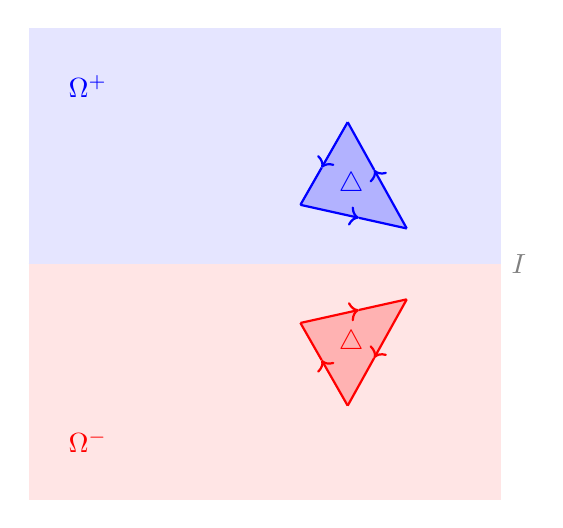
\begin{tikzpicture}[scale=1.5]
            % Draw the real axis I
            \draw[thick, dashed, gray] (-2,0) -- (2,0) node[right] {$I$};
            \node[below] at (0,-0.1) {$\Im(z)=0$};
            
            % Draw Omega^+ region (upper half-plane)
            \fill[blue!10] (-2,0) -- (2,0) -- (2,2) -- (-2,2) -- cycle;
            \node[blue] at (-1.5,1.5) {$\Omega^+$};
            
            % Draw Omega^- region (lower half-plane)
            \fill[red!10] (-2,0) -- (2,0) -- (2,-2) -- (-2,-2) -- cycle;
            \node[red] at (-1.5,-1.5) {$\Omega^-$};
            
            % Case 1a: Triangle in Omega^+
            \coordinate (A1) at (0.3,0.5);
            \coordinate (B1) at (1.2,0.3);
            \coordinate (C1) at (0.7,1.2);
            \fill[blue!30] (A1) -- (B1) -- (C1) -- cycle;
            \draw[thick, blue, ->] (A1) -- ($(A1)!0.55!(B1)$);
            \draw[thick, blue] ($(A1)!0.55!(B1)$) -- (B1);
            \draw[thick, blue, ->] (B1) -- ($(B1)!0.55!(C1)$);
            \draw[thick, blue] ($(B1)!0.55!(C1)$) -- (C1);
            \draw[thick, blue, ->] (C1) -- ($(C1)!0.55!(A1)$);
            \draw[thick, blue] ($(C1)!0.55!(A1)$) -- (A1);
            \node[blue] at (0.73,0.67) {$\triangle$};
            
            % Case 1b: Triangle in Omega^- (on the right side)
            \coordinate (A2) at (0.3,-0.5);
            \coordinate (B2) at (1.2,-0.3);
            \coordinate (C2) at (0.7,-1.2);
            \fill[red!30] (A2) -- (B2) -- (C2) -- cycle;
            \draw[thick, red, ->] (A2) -- ($(A2)!0.55!(B2)$);
            \draw[thick, red] ($(A2)!0.55!(B2)$) -- (B2);
            \draw[thick, red, ->] (B2) -- ($(B2)!0.55!(C2)$);
            \draw[thick, red] ($(B2)!0.55!(C2)$) -- (C2);
            \draw[thick, red, ->] (C2) -- ($(C2)!0.55!(A2)$);
            \draw[thick, red] ($(C2)!0.55!(A2)$) -- (A2);
            \node[red] at (0.73,-0.67) {$\triangle$};
        \end{tikzpicture}
    \end{center}
    \textbf{Case 2:} If a vertex or side of $\triangle$ is on $I$, $\int_{\partial \triangle_\epsilon}f=0$ for when $\epsilon\to 0, \partial \triangle_\epsilon\to \partial \triangle$.
    \begin{center}
        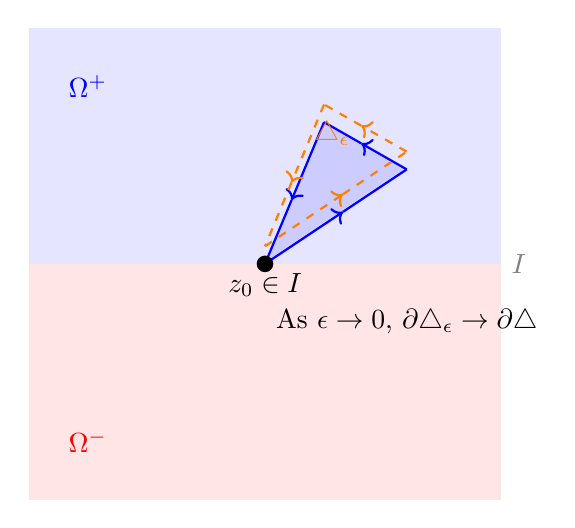
\begin{tikzpicture}[scale=1.5]
            % Draw the real axis I
            \draw[thick, dashed, gray] (-2,0) -- (2,0) node[right] {$I$};
            \node[below] at (0,-0.1) {$\Im(z)=0$};
            
            % Draw Omega^+ region
            \fill[blue!10] (-2,0) -- (2,0) -- (2,2) -- (-2,2) -- cycle;
            \node[blue] at (-1.5,1.5) {$\Omega^+$};
            
            % Draw Omega^- region
            \fill[red!10] (-2,0) -- (2,0) -- (2,-2) -- (-2,-2) -- cycle;
            \node[red] at (-1.5,-1.5) {$\Omega^-$};
            
            % Triangle with vertex on I
            \coordinate (A) at (0,0);
            \coordinate (B) at (1.2,0.8);
            \coordinate (C) at (0.5,1.2);
            
            % Draw the original triangle (partially in Omega^+)
            \fill[blue!20] (A) -- (B) -- (C) -- cycle;
            \draw[thick, blue, ->] (A) -- ($(A)!0.55!(B)$);
            \draw[thick, blue] ($(A)!0.55!(B)$) -- (B);
            \draw[thick, blue, ->] (B) -- ($(B)!0.55!(C)$);
            \draw[thick, blue] ($(B)!0.55!(C)$) -- (C);
            \draw[thick, blue, ->] (C) -- ($(C)!0.55!(A)$);
            \draw[thick, blue] ($(C)!0.55!(A)$) -- (A);
            
            % Mark the vertex on I
            \fill[black] (A) circle (2pt);
            \node[below] at (A) {$z_0 \in I$};
            
            % Draw the perturbed triangle triangle_epsilon (shifted slightly up)
            \coordinate (Aeps) at (0,0.15);
            \coordinate (Beps) at (1.2,0.95);
            \coordinate (Ceps) at (0.5,1.35);
            
            \draw[thick, orange, dashed, ->] (Aeps) -- ($(Aeps)!0.55!(Beps)$);
            \draw[thick, orange, dashed] ($(Aeps)!0.55!(Beps)$) -- (Beps);
            \draw[thick, orange, dashed, ->] (Beps) -- ($(Beps)!0.55!(Ceps)$);
            \draw[thick, orange, dashed] ($(Beps)!0.55!(Ceps)$) -- (Ceps);
            \draw[thick, orange, dashed, ->] (Ceps) -- ($(Ceps)!0.55!(Aeps)$);
            \draw[thick, orange, dashed] ($(Ceps)!0.55!(Aeps)$) -- (Aeps);
            \node[orange] at (0.57,1.1) {$\triangle_\epsilon$};
            
            \node[below] at (1.2,-0.3) {As $\epsilon \to 0$, $\partial \triangle_\epsilon \to \partial \triangle$};
        \end{tikzpicture}
    \end{center}
    \textbf{Case 3:} If $I$ cuts the triangle then we can split the triangle into smaller triangles and we're done.
    \begin{center}
        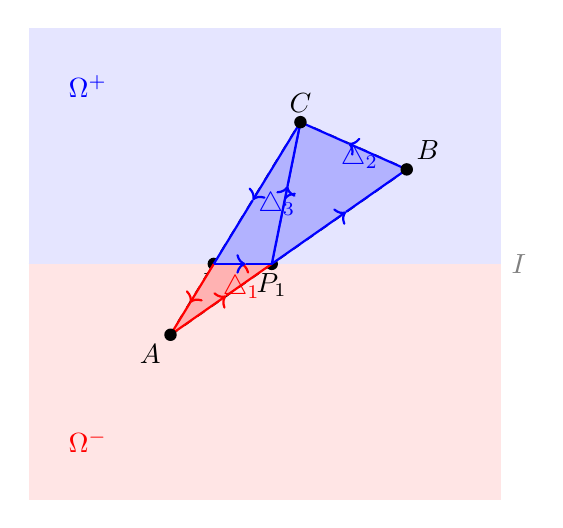
\begin{tikzpicture}[scale=1.5]
            % Draw the real axis I
            \draw[thick, dashed, gray] (-2,0) -- (2,0) node[right] {$I$};
            \node[below] at (0,-0.1) {$\Im(z)=0$};
            
            % Draw Omega^+ region
            \fill[blue!10] (-2,0) -- (2,0) -- (2,2) -- (-2,2) -- cycle;
            \node[blue] at (-1.5,1.5) {$\Omega^+$};
            
            % Draw Omega^- region
            \fill[red!10] (-2,0) -- (2,0) -- (2,-2) -- (-2,-2) -- cycle;
            \node[red] at (-1.5,-1.5) {$\Omega^-$};
            
            % Original triangle that crosses I
            \coordinate (A) at (-0.8,-0.6);
            \coordinate (B) at (1.2,0.8);
            \coordinate (C) at (0.3,1.2);
            
            % Draw the original triangle outline
            \draw[thick, black, dashed] (A) -- (B) -- (C) -- cycle;
            
            % Find intersection points with I (the real axis at y=0)
            % Line AB: from (-0.8,-0.6) to (1.2,0.8)
            % Parametric: (-0.8,-0.6) + t*(2.0,1.4), t such that y=0: -0.6 + 1.4t = 0 => t = 0.6/1.4 = 3/7
            \coordinate (P1) at ({-0.8 + 3/7*2.0}, 0);
            
            % Line AC: from (-0.8,-0.6) to (0.3,1.2)
            % Parametric: (-0.8,-0.6) + t*(1.1,1.8), t such that y=0: -0.6 + 1.8t = 0 => t = 1/3
            \coordinate (P2) at ({-0.8 + 1/3*1.1}, 0);
            
            % Mark intersection points
            \fill[black] (P1) circle (1.5pt);
            \fill[black] (P2) circle (1.5pt);
            \node[below] at (P1) {$P_1$};
            \node[below] at (P2) {$P_2$};
            
            % Split into triangles
            % Triangle 1: A, P1, P2 (in Omega^-)
            \fill[red!30] (A) -- (P1) -- (P2) -- cycle;
            \draw[thick, red, ->] (A) -- ($(A)!0.55!(P1)$);
            \draw[thick, red] ($(A)!0.55!(P1)$) -- (P1);
            \draw[thick, red, ->] (P1) -- ($(P1)!0.55!(P2)$);
            \draw[thick, red] ($(P1)!0.55!(P2)$) -- (P2);
            \draw[thick, red, ->] (P2) -- ($(P2)!0.55!(A)$);
            \draw[thick, red] ($(P2)!0.55!(A)$) -- (A);
            \node[red] at (-0.2,-0.2) {$\triangle_1$};
            
            % Triangle 2: P1, B, C (in Omega^+)
            \fill[blue!30] (P1) -- (B) -- (C) -- cycle;
            \draw[thick, blue, ->] (P1) -- ($(P1)!0.55!(B)$);
            \draw[thick, blue] ($(P1)!0.55!(B)$) -- (B);
            \draw[thick, blue, ->] (B) -- ($(B)!0.55!(C)$);
            \draw[thick, blue] ($(B)!0.55!(C)$) -- (C);
            \draw[thick, blue, ->] (C) -- ($(C)!0.55!(P1)$);
            \draw[thick, blue] ($(C)!0.55!(P1)$) -- (P1);
            \node[blue] at (0.8,0.9) {$\triangle_2$};
            
            % Triangle 3: P2, P1, C (in Omega^+)
            \fill[blue!30] (P2) -- (P1) -- (C) -- cycle;
            \draw[thick, blue, ->] (P2) -- ($(P2)!0.55!(P1)$);
            \draw[thick, blue] ($(P2)!0.55!(P1)$) -- (P1);
            \draw[thick, blue, ->] (P1) -- ($(P1)!0.55!(C)$);
            \draw[thick, blue] ($(P1)!0.55!(C)$) -- (C);
            \draw[thick, blue, ->] (C) -- ($(C)!0.55!(P2)$);
            \draw[thick, blue] ($(C)!0.55!(P2)$) -- (P2);
            \node[blue] at (0.1,0.5) {$\triangle_3$};
            
            % Mark vertices
            \fill (A) circle (1.5pt) node[below left] {$A$};
            \fill (B) circle (1.5pt) node[above right] {$B$};
            \fill (C) circle (1.5pt) node[above] {$C$};
        \end{tikzpicture}
    \end{center}
    The triangle is split into smaller triangles, each either entirely in $\Omega^+$ or $\Omega^-$, or with edges on $I$, so we can apply Cases 1 and 2.
\end{proof}
\begin{thm}
    Schwarz Reflection Principle: Let $f:\Omega^+\to \C$ be holomorphic and extend continuous to $I$ with $f^+/I\in \R$ then $f^+$ extends analytically to $\Omega$
\end{thm}
\begin{proof}
    Let $f^-:\Omega^-\to \C$ be defined by $f^-(z)=\overline{f^+(\overline{z})}$. We claim $f^-$ is holomorphic on $\Omega^-$, then the previous theorem applies because $f^+=f^-$ on $I.$\\
    Fix $z_0\in \Omega^-$ then $\overline{z_0}\in \Omega^+$, we know $f^+(\overline{z})=\sum_{n=0}^{\infty}a_n(\overline{z}-\overline{z_0})^n$ for all $\overline{z}\in D(\overline{z_0})$. Thus \[
    \overline{f^+(\overline{z})}=\sum_{n=0}^\infty \overline{a_n}(\overline{z}-\overline{z_0})^n
    .\] 
    We know $\overline{\overline{z}-\overline{z_0}}=z-z_0$ so \[
    f^-(z)=\overline{f^+(\overline{z})}=\sum\overline{a_n}(z-z_0)^n
    .\] 
\end{proof}
\newpage
\section{Feb 9}
\begin{defn}
    Meromorphic functions are "determined" by zeros and singularities. \\
    A point singulaity of $f$ is a point $z_0\in \C$ such that $f$ is defined in a neighborhood of $z_0$ but not at $z_0$. \[
    \mathcal{D}_\delta(z_0)\setminus \{z_0\}
    .\] 
\end{defn}
\begin{eg}
    $f(z)=\frac{1}{z}$ has a singularity at $z_0=0$.
\end{eg}
\begin{rmk}
    Zeros of a holomorphic $f$ are isolated, unless $f\equiv 0$.
\end{rmk}
\begin{thm}
    (Local Description Near Zeros) Let $f:\substack{\Omega}_{ \text{open}}\to \C$ holomorphic and $f(z_0)=0$, $z_0\in \Omega, f\not \equiv 0$ then   
\end{thm}
\end{document}
